\documentclass[12pt]{article}
\usepackage{amsmath}
\usepackage{amssymb}
\usepackage{amsthm}
\usepackage{booktabs}
\usepackage{enumerate}
\usepackage{enumitem}
\usepackage{float}
%\usepackage{footnote}
%\usepackage[bottom]{footmisc}
\usepackage[singlelinecheck=false]{caption}

\usepackage{graphicx,psfrag,epsf}
\usepackage[space]{grffile}
\usepackage{natbib}
\usepackage{url} % not crucial - just used below for the URL 

%\pdfminorversion=4
% NOTE: To produce blinded version, replace "0" with "1" below.
\newcommand{\blind}{1}

% DON'T change margins - should be 1 inch all around.
\addtolength{\oddsidemargin}{-.5in}%
\addtolength{\evensidemargin}{-.5in}%
\addtolength{\textwidth}{1in}%
\addtolength{\textheight}{1.3in}%
\addtolength{\topmargin}{-.8in}%

\newtheorem{theorem}{Theorem}
\newtheorem{lemma}{Lemma}
\newtheorem{claim}{Claim}
\newtheorem{proposition}{Proposition}
\newtheorem{definition}{Definition}
\newtheorem{corollary}{Corollary}

% operators
\DeclareMathOperator*{\argmin}{arg\,min}
\newcommand{\CV}{\operatorname{CV}}
\newcommand{\PE}{\operatorname{PE}}
\newcommand{\E}{\operatorname{E}}
\DeclareMathOperator*{\cov}{cov}
\DeclareMathOperator*{\cor}{cor}
\DeclareMathOperator*{\tr}{tr}
\DeclareMathOperator*{\var}{var}
\newcommand{\T}{T}

% convergence
\newcommand{\toas}{\overset{\mathit{a.s.}}{\to}}

\newcommand{\Oh}{O}
\newcommand{\OhP}{O_p}

% sets
\newcommand{\R}{\mathbb{R}}
\newcommand{\sA}{\mathcal{A}}
\newcommand{\sbA}{\mathcal{\bar A}}
\newcommand{\sC}{\mathcal{C}}
\newcommand{\sE}{\mathcal{E}}
\newcommand{\sN}{\mathcal{N}}
\newcommand{\sX}{\mathcal{X}}

% scalars
\newcommand{\bpi}{\bar \pi}

% vectors
\newcommand{\muX}{\mu^{X}}
\newcommand{\muY}{\mu^{Y}}
\newcommand{\bmuX}{\bar \mu^{X}}
\newcommand{\bmuY}{\bar \mu^{Y}}
\newcommand{\hmuY}{\hat \mu^{Y}}

% matrices
\newcommand{\dataX}{\mathfrak{X}}
\newcommand{\SigmaY}{\Sigma^Y}
\newcommand{\Xtrain}{X_{\text{train}}}
\newcommand{\Ytrain}{Y_{\text{train}}}
\newcommand{\Xtest}{X_{\text{test}}}
\newcommand{\Ytest}{Y_{\text{test}}}

% class labels
\newcommand{\hGX}{\hat G^{X}}
\newcommand{\hGY}{\hat G^{Y}}

\begin{document}

%\bibliographystyle{natbib}

\def\spacingset#1{\renewcommand{\baselinestretch}%
{#1}\small\normalsize} \spacingset{1}


%%%%%%%%%%%%%%%%%%%%%%%%%%%%%%%%%%%%%%%%%%%%%%%%%%%%%%%%%%%%%%%%%%%%%%%%%%%%%%

\if1\blind
{
  \title{\bf Supplement to ``Estimating the number of clusters using
cross-validation''}
  \author{Wei Fu and Patrick O. Perry \\
  Stern School of Business, New York University}
  \maketitle
} \fi

\if0\blind
{
  \bigskip
  \bigskip
  \bigskip
  \begin{center}
    {\LARGE\bf Estimating the number of clusters using cross-validation}
\end{center}
  \medskip
} \fi

\bigskip

\spacingset{1.45} % DON'T change the spacing!

\section{Clustering scree plot examples}

\label{sec:elbow-fail}

The top row of Figure~\ref{fig:elbow}
displays an example where the elbow in $W_k$ corresponds to the true number $k
= 4$ of mixture components in the data-generating mechanism. The elbow
approach is simple and often performs well, but it requires subjective
judgment as to where the elbow is located, and, as the bottom row of
Figure~\ref{fig:elbow} demonstrates, the approach can easily fail.

\begin{figure}
\centering
\begin{minipage}{\linewidth}
  \begin{minipage}{0.45\linewidth}
    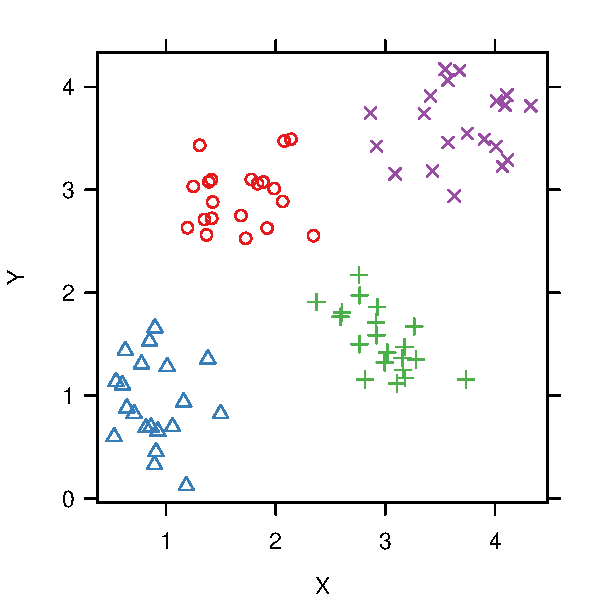
\includegraphics[width=\linewidth]{main_code/demo/elbow/correct-data.pdf}
  \end{minipage}
  \hspace{0.05in}
  \begin{minipage}{0.45\linewidth}
    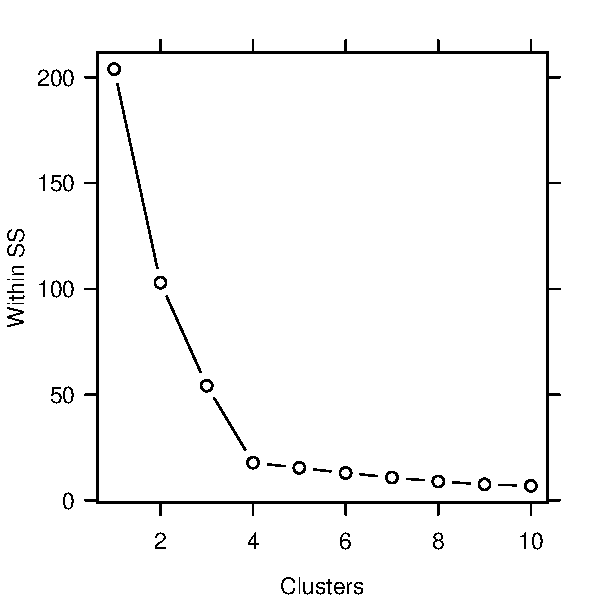
\includegraphics[width=\linewidth]{main_code/demo/elbow/correct-withinss.pdf}
  \end{minipage}
\end{minipage}
\begin{minipage}{\linewidth}
  \begin{minipage}{0.45\linewidth}
    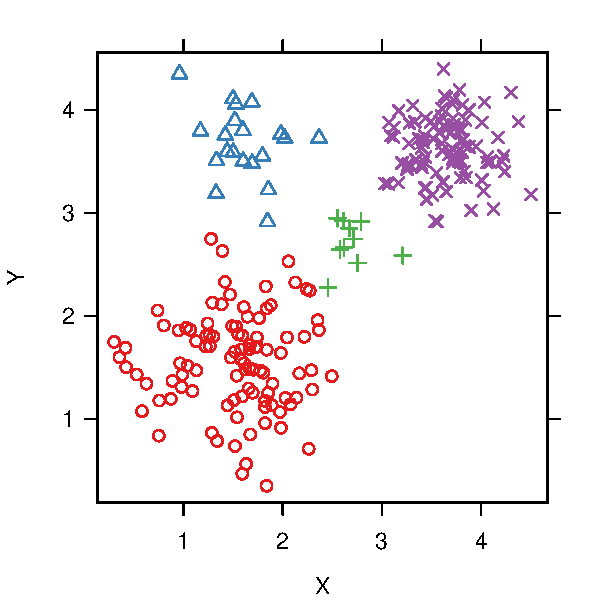
\includegraphics[width=\linewidth]{main_code/demo/elbow/incorrect-data.pdf}
  \end{minipage}
  \hspace{0.05in}
  \begin{minipage}{0.45\linewidth}
    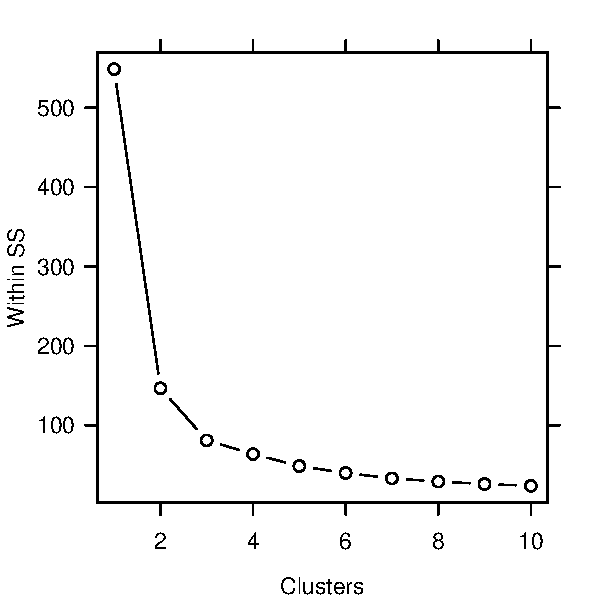
\includegraphics[width=\linewidth]{main_code/demo/elbow/incorrect-withinss.pdf}
  \end{minipage}
\end{minipage}
\caption{Scree plots for two data sets. Left panels show the sets of
    two-dimensional data points, generated from four clusters, with plotting
    symbol indicating the generated cluster. Right panels show the
    corresponding values of the within-cluster sum of squares $W_k$
    plotted against the number of clusters, $k$. The scree plot identifies
    the correct number of clusters in the top row, but fails in the bottom
    row.}
\label{fig:elbow}
\end{figure}


\section{Self-consistency}
\label{sec:self-consistent}

An important property of any estimation procedure is that in the absence of
noise, the procedure correctly estimates the truth. This property is called
``self-consistency'' \citep{tarpey96}. We will now show that Gabriel
cross-validation is self-consistent. That is, in the absence of noise, the
Gabriel cross-validation procedure finds the optimal number of clusters.


Self-consistency by itself does not mean that a procedure performs well in
practice. Self-consistency deals only with the no-noise situation.  Many other
methods for selecting $K$ are likely self-consistent, but not all perform the
same in practice. Self-consistency only suggests (but does not guarantee) that
a procedure might perform reasonably when the noise level is low.


It will suffice to prove self-consistency for a single fold of the
cross-validation procedure.  As in section~\ref{sec:gabriel-cv-algorithm} we
assume that the $P$ variables of the data set have been partitioned into $p$
predictor variables represented in vector~$X$ and $q$ response variables
represented in vector~$Y$.  The $N$ observations have been divided into two
sets: $n$ train observations and $m$ test observations.  We state the
assumptions for the self-consistency result in terms of a specific split; for
the result to hold in general, with high probability, these assumptions would
have to hold with high probability for a random split. The following theorem
gives conditions for Gabriel cross-validation to recover the true number of
clusters in the absence of noise.


\begin{proposition}\label{prop:self-consistency}

Let $\{ (X_i, Y_i) \}_{i=1}^{n+m}$ be the data from a single fold of Gabriel
cross-validation.  For any $k$, let $\CV(k)$ be the cross-validation error for
this fold, computed as described in Section~\ref{sec:gabriel-cv-algorithm}.
We will assume that there are $K$ ``true cluster centers''
$\mu(1), \dotsc,\mu(K)$, with
the $g$th cluster center partitioned as $\mu(g) = \bigl(\muX(g),
\muY(g)\bigr)$ for $g = 1, \dotsc, K$.  Suppose that
\begin{enumerate}[label=(\roman*)]
  \item \label{asn:self-consistency-noiseless}
    Each observation $i$ has a true cluster $G_i \in \{ 1, \dotsc, K \}$.
    There is no noise, so that $X_i = \muX({G_i})$ and $Y_i = \muY(G_i)$ for
    $i = 1, \dotsc, n+m$.
  \item \label{asn:self-consistency-distinct-mux}
    The vectors $\muX(1), \dotsc,\muX(K)$ are all distinct.
  \item \label{asn:self-consistency-distinct-muy}
    The vectors $\muY(1), \dotsc,\muY(K)$ are all distinct.
  \item \label{asn:self-consistency-train}
    The training set contains at least one member of each cluster: for all $g$
    in the range $1, \dotsc, K$, there exists at least one $i$ in the range
    $1, \dotsc, n$ such that $G_i = g$.
  \item \label{asn:self-consistency-test}
    The test set contains at least one member of each cluster: for all $g$ in
    the range $1, \dotsc, K$, there exists at least one $i$ in the range $n+1,
    \dotsc, n+m$ such that $G_i = g$.
\end{enumerate}
Then $\CV(k) > \CV(K)$ for $k < K$, and $\CV(k) = \CV(K)$ for $k > K$, so that
Gabriel cross-validation correctly chooses $k = K$.
\end{proposition}

The proposition states that our method works well in the absence of noise,
when each observation is equal to its cluster center.  The assumptions here
are not checkable in practice, but the proposition suggest that Gabriel
cross-validation might give a reasonable answer, at least when the noise level
is low.

The essential
assumption here is assumption~\ref{asn:self-consistency-noiseless}, which states
that there is no noise.  If we are willing to assume, say, that the cluster
centers~$\mu(g) = \bigl(\muX(g),\muY(g)\bigr)$ for $g = 1, \dotsc, K$ were
randomly drawn from a distribution with a density over $\R^{p+q}$, then
assumptions~\ref{asn:self-consistency-distinct-mux}
and~\ref{asn:self-consistency-distinct-muy} will hold with probability one for
all splits of the data. Likewise, if the clusters are not too small (relative
to $n$ and $m$), then assumptions~\ref{asn:self-consistency-train}
and~\ref{asn:self-consistency-test} will likely hold for a random split of the
data into test and train.


Proposition~\ref{prop:self-consistency} follows from
Lemmas~\ref{lem:self-consistency1} and~\ref{lem:self-consistency2}, which we
now state and prove.


\begin{lemma}\label{lem:self-consistency1}
Suppose that the assumptions of Proposition~\ref{prop:self-consistency} are in
force.  If $k < K$, then $\CV(k) > 0$.
\end{lemma}
\begin{proof}
By definition,
\[
  \CV(k)
    =
      \sum_{i=n+1}^{n+m}
        \| Y_i - \bmuY (\hGX_i) \|^2,
\]
where $\bmuY(g)$ is the center of cluster $g$ returned from applying $k$-means
to $Y_1, \dotsc, Y_n$.  Assumptions~\ref{asn:self-consistency-noiseless}
and~\ref{asn:self-consistency-test}, imply that as $i$ ranges over the test
set $n+1, \dotsc, n+m$, the response $Y_i$ ranges over all distinct values in
$\{ \muY(1), \dotsc, \muY(K) \}$.
Assumption~\ref{asn:self-consistency-distinct-muy} implies that there are
exactly $K$ such distinct values.  However, there are only $k$ distinct values
of $\bmuY(g)$.  Thus, at least one summand
\(
  \| Y_i - \bmuY(\hGX_i) \|^2
\)
is nonzero.  Therefore,
\(
  \CV(k) > 0.
\)
\end{proof}

\begin{lemma}\label{lem:self-consistency2}
Suppose that the assumptions of Proposition~\ref{prop:self-consistency} are in
force.  If $k \geq K$, then $\CV(k) = 0$.
\end{lemma}
\begin{proof}
From assumptions~\ref{asn:self-consistency-noiseless},
\ref{asn:self-consistency-distinct-muy},
and~\ref{asn:self-consistency-train}, we know the cluster centers
gotten from applying $k$-means to $Y_1, \dotsc, Y_n$ must include
$\muY(1), \dotsc, \muY(K)$.  Without loss of generality, suppose that
$\bmuY(g) = \muY(g)$ for $g = 1, \dotsc, K$.  This implies that
$\hGY_i = G_i$ for $i = 1, \dotsc, n$.  Thus, employing
assumption~\ref{asn:self-consistency-noiseless} again, we get that
$\bmuX(g) = \muX(g)$ for $g = 1, \dotsc, K$.


Since assumption~\ref{asn:self-consistency-distinct-mux} ensures that
$\muX(1), \dotsc, \muX(K)$ are all distinct, we must have that $\hGX_i = G_i$
for all $i = 1, \dotsc, m+n$.  In particular, this implies that $\bmuY(\hGX_i)
= Y_i$ for $i = 1, \dotsc, m+n$, so that $\CV(k) = 0$.
\end{proof}


%% \section{Review of consistency results for clustering}
%% 
%% Some proposed methods provide theoretical consistency result for choosing $k$.
%% Assume data is a mixture of $G$ $p$-dimension clusters with equal prior,
%% identically distributed with common covariance matrix and finite fourth
%% moments in each dimension, \citet{sugar2003finding} shows the Jump method will
%% pick the correct $k$ under the conditions that cluster centers are
%% sufficiently separated and an appropriate transformation is used.
%% Specifically, let $\Delta\sqrt{p}$ denotes the minimum Euclidean distance
%% between cluster centers, \citet{sugar2003finding} shows that the jump will be
%% maximized at $k=G$ given that $\Delta > 6$ and the existence of a positive $Y$
%% such that
%% \[
%%   \left(\frac{p\Delta^2W}{9G}\right)^{-Y}
%%     + \left(
%%         W \left[\frac{2^{2H^*(X)}}{K^2_{max}2\pi e}\right]
%%         - (\frac{\Delta}{6})^2(1-W)
%%       \right)^{-Y} < 2
%% \]
%% and $\left(\frac{p\Delta^2W}{9G}\right)^{-Y} <1/2$, where $H^*(X)$ is the
%% minimum entropy of the cluster membership over each dimension and $W =1-
%% \frac{6^4V_{\mathbf{X}}}{(\Delta^2-36)^2}$ with $V_{\mathbf{X}} = \var\left(
%%   1/p ||\mathbf{X}-\mu_j||^2_{\Gamma^{-1}} \mid \mathbf{X}
%% \hspace{0.05in}\text{in jth cluster}\right)$
%% 
%% \cite{tibshirani2005cluster} proved that the prediction strength method is
%% consistent under the setting that the observations in $p$-dimension are
%% uniformly distributed within one unit from their respective cluster centers,
%% with minimum distance between the $G$ cluster centers is four unit. Under such
%% well-separated setting, they show that 
%% \[ ps(G) = 1+ o_p(1), \hspace{0.5in} \underset{k \geq G+1}{\text{sup}} ps(k)\leq \frac{2}{3}+ o_p(1) \]
%% therefore $\hat{k}$ is consistent in estimating $G$.  When data does come from
%% mixture of Gaussian distribution, the model-based method of
%% \citet{fraley2002model} is consistent in estimating $k$ in low dimension.
%% 
%% Let $\Psi$ denotes any given base-clustering algorithm (e.g $k$-means), and
%% $\Psi(Z,k)$ the clustering obtained by applying $\Psi$ on data $Z$ with
%% parameter $k$. Also let $k_0$ be the optimal number of cluster and
%% $d\{\Psi(Z_1,k),\Psi(Z_2,k)\}$ be the measure of distance between clustering
%% $\Psi(Z_1,k)$ and $\Psi(Z_2,k)$ where $Z_1$ and $Z_2$ are two independent
%% samples from population. \citet{wang2010consistent} shows that their proposed
%% method will consistently select $k = k_0$, given such $k_0$ exists and
%% $d\{\Psi(Z_1,k),\Psi(Z_2,k)\}$ converges to zero at proper rate $r_k$.
%% However, $k_0$ is defined as the most stable number for $\Psi$ among all the
%% possible $k$, instead of the number of components in mixture model or
%% well-separated compact regions commonly seen in literature. Therefore, their
%% consistent result actually is convergent result, i.e. the selected $k$
%% converges to its limit $k_0$ given such limit exists.



\section{Analysis of single cluster in more than two dimensions}
\label{sec:single-general-dim}

\begin{proposition}\label{prop:single-general-dim}
Suppose that $\{ (X_i, Y_i) \}_{i=1}^{n + m}$ is data from a single fold
of Gabriel cross-validation, where each $(X,Y)$ pair in $\R^{p+q}$ is an
independent draw from a mean-zero multivariate normal distribution with 
covariance matrix $\Sigma = \left( \begin{smallmatrix} \Sigma_{XX} & \Sigma_{XY} \\ 
 \Sigma_{YX} & \Sigma_{YY} \end{smallmatrix}\right)$, with $\Sigma_{YY}$ has leading 
eigenvalue $\lambda_1$ and corresponding eigenvector $u_1$. In this case, the data are drawn
from a single cluster; the true number of clusters is~$1$.  If  $\frac{\sqrt{\lambda_1}}{2}
 > \frac{u^T_1\Sigma_{YX}\Sigma_{XY}u_1}{\sqrt{u^T_1\Sigma_{YX} \Sigma_{XX} \Sigma_{XY} u_1}}$,
then $\CV(1) < \CV(2)$ with probability tending to one as $m$ and $n$ increase.
\end{proposition}

\begin{proof}
Let $X$ and $Y$ be jointly multivariate normal distributed with mean $\mathbf{0}$ and covariance matrix $\Sigma$, i.e.
\[	(X,Y) \sim \mathcal{N} \left( \mathbf{0}, \Sigma\right)	\]
where $\Sigma=\begin{bmatrix} \Sigma_{XX} & \Sigma_{XY} \\  \Sigma_{YX} & \Sigma_{YY} \end{bmatrix}$.

Let $\Sigma_{YY} = U \Lambda U^T$  be the eigendecomposition of $\Sigma_{YY}$,
with leading eigenvalue $\lambda_1$ and corresponding eigenvector $u_1$. Then
the centroid of $k$-means applying on $(y_1,..,y_n)$ is on the first principal
component
of $Y$,\[	E(u^T_1 Y|u^T_1 Y>0) = \bar{\mu}^Y_1 =\sqrt{2 \lambda_1/\pi}u_1\] and 
\[	E(u^T_1 Y|u^T_1 Y<0) = \bar{\mu}^Y_2 =-\sqrt{2 \lambda_1/\pi}u_1\]
 where $u^T_1 Y \sim \mathcal{N}(0,\lambda_1)$.

To compute $\bar{\mu}^X_1 = E(X|u^T_1 Y>0)$, we need to know the conditional distribution $X|u^T_1 Y$. Since $(X,Y)$ has multivariate normal distribution, $(X,u^T_1 Y)$ also has a multivariate normal distribution with mean $\mathbf{0}$ and covariance matrix
$$\Sigma_{X,u^T_1 Y}=\begin{bmatrix} \Sigma_{XX} & \Sigma_{XY} u_1 \\  u^T_1 \Sigma_{YX} & \lambda_1 \end{bmatrix}$$
The conditional distribution $X|u^T_1 Y$ is hence normal with mean
 $$\mu_{X|u^T_1 Y} = \Sigma_{XY} u_1 \lambda^{-1}_1 u^T_1 Y $$
Therefore, 
\begin{align}
\bar{\mu}^X_1 &= E(X \mid u^T_1 Y>0) \nonumber \\ \nonumber
 			  &= E\left(E[X \mid u^T_1 Y] \mid u^T_1 Y>0\right) \\ \nonumber
 			  &=  E\left(\Sigma_{XY} u_1 \lambda^{-1}_1 u^T_1 Y \mid u^T_1 Y>0\right)\\ \nonumber
 			  &= \lambda^{-1}_1 \Sigma_{XY}u_1 E(u^T_1 Y \mid u^T_1 Y>0) \\ \nonumber
 			  &= \lambda^{-1}_1 \Sigma_{XY}u_1 \sqrt{2 \lambda_1/\pi} \\ \nonumber
      &= \sqrt{2 / (\lambda_1 \pi)} \Sigma_{XY}u_1
\end{align}
Similar calculation yields $\bar{\mu}^X_2 = -\sqrt{2 / (\lambda_1 \pi)} \Sigma_{XY}u_1$.
The decision rule to classify any observed value of $X$ to $\bar{\mu}^X_1$ is therefore
\[	(\bar{\mu}^X_1)^T X >0	\hspace{0.2in}\text{or} \hspace{0.2in} u^T_1\Sigma_{YX}X>0\] 
Since $u^T_1\Sigma_{YX}X$ is a linear combination of $X$, it also has normal distribution 
\[	\mathcal{N} \left( 0, u^T_1\Sigma_{YX} \Sigma_{XX} \Sigma_{XY} u_1\right)	\]
And $(Y,u^T_1\Sigma_{YX}X)$ also have multivariate normal distribution with mean $\mathbf{0}$ 
and covariance matrix
\[
\begin{bmatrix}
\Sigma_{YY} & \Sigma_{YX}\Sigma_{XY}u_1  \\
u^T_1\Sigma_{YX}\Sigma_{XY} &  u^T_1\Sigma_{YX} \Sigma_{XX} \Sigma_{XY} u_1
\end{bmatrix}
\]
The conditional distribution of $Y|u^T_1\Sigma_{YX}X$ is also multivariate normal with mean 
\[	
\mu_{Y|u^T_1\Sigma_{YX}X } = \Sigma_{YX}\Sigma_{XY}u_1 (u^T_1\Sigma_{YX} \Sigma_{XX} \Sigma_{XY} u_1)^{-1}u^T_1\Sigma_{YX}X	
\]
The $Y$ center for $u^T_1\Sigma_{YX}X>0$ is
\begin{align}
\hat{\mu}^Y_1 &= E(Y|u^T_1\Sigma_{YX}X>0) \nonumber \\ \nonumber
 		      & =  \Sigma_{YX}\Sigma_{XY}u_1 (u^T_1\Sigma_{YX} \Sigma_{XX} \Sigma_{XY} u_1)^{-1} E(u^T_1\Sigma_{YX}X \mid u^T_1\Sigma_{YX}X>0) \\ \nonumber
\end{align}
Note that $u^T_1\Sigma_{YX}X$ has normal distribution $\mathcal{N} \left( 0, u^T_1\Sigma_{YX} \Sigma_{XX} \Sigma_{XY} u_1\right)$, so
\[
E(u^T_1\Sigma_{YX}X \mid u^T_1\Sigma_{YX}X>0) = \sqrt{2/\pi}\cdot\sqrt{u^T_1\Sigma_{YX} \Sigma_{XX} \Sigma_{XY} u_1}
\]
Therefore, we have the $Y$ center for $u^T_1\Sigma_{YX}X>0$ be
\begin{align*}
\hat{\mu}^Y_1 &= \sqrt{2/\pi}\cdot\sqrt{u^T_1\Sigma_{YX} \Sigma_{XX} \Sigma_{XY} u_1} \hspace{0.1in} \Sigma_{YX}\Sigma_{XY}u_1 (u^T_1\Sigma_{YX} \Sigma_{XX} \Sigma_{XY} u_1)^{-1} \\
&=\frac{\sqrt{2/\pi}}{\sqrt{u^T_1\Sigma_{YX} \Sigma_{XX} \Sigma_{XY} u_1}} \Sigma_{YX}\Sigma_{XY}u_1
\end{align*} 
 
Recall that $\bar{\mu}^Y_1 =\sqrt{2 \lambda_1/\pi}u_1$, to judge if $\CV(2) >
\CV(1)$, one only need to compare the distance between  $\hat{\mu}^Y_1$  and
$\bar{\mu}^Y_1$ with distance between  $\hat{\mu}^Y_1$ and grand mean $0$. By
the variance and bias decomposition of prediction MSE, when variance is the
same, only bias influences the MSE. 

After some linear algebra manipulation, we get
$\|\hat{\mu}^Y_1 - \bar{\mu}^Y_1\|^2 > \|\hat{\mu}^Y_1\|^2$ or $\CV(2) >
\CV(1)$ if and only if
\[
 \frac{\sqrt{\lambda_1}}{2} > \frac{u^T_1\Sigma_{YX}\Sigma_{XY}u_1}{\sqrt{u^T_1\Sigma_{YX} \Sigma_{XX} \Sigma_{XY} u_1}} 
\]
\end{proof}


The condition that ensures $\CV(1) < \CV(2)$ is tight but difficult to
understand intuitively. We make understand this condition better by
noting that it is equivalent to a condition on the correlation between the
two linear combinations of $X$ and $Y$ variables:
\begin{equation}\label{eqn:clust-anyd}
    \cor(u_1^\T \Sigma_{YX} X, u_1^\T Y) < 1/2.
\end{equation}
A stronger condition that is easier to understand, then, is that the canonical
correlation between $X$ and $Y$ is below $1/2$; when the latter is true the
former follows and $\CV(1) < \CV(2)$. A necessary but not sufficient
guarantee of the stronger condition is that all correlations between variables
are below $1/2$.


One might object to the condition~\eqref{eqn:clust-anyd} being stated in terms
of a particular $(X, Y)$ split of the data.  In practice, one might want the
condition to hold for all possible splits of the data. A sufficient guarantee
that~\eqref{eqn:clust-anyd} holds for any $(X, Y)$ split of the data is that
the data covariance matrix $\Sigma$ is diagonal. The ad-hoc adjustment we
propose in Sec.~\ref{sec:corr-correct} attempts to transform the data to this
form.



\section{Analysis of two clusters in more than two dimensions}
\label{app:twoclust-anyd}


\begin{proposition}\label{prop:twoclust-anyd}
Suppose that $\{(X_i,Y_i)\}_{i=1}^{n+m}$ is data from a single fold of Gabriel
    cross-validation, where each $(X,Y)$ pair in with $X \in \mathbb{R}^P$ and $Y \in
    \mathbb{R}^Q$ is an independent draw
from an equiprobable mixture of two multivariate normal distributions with
identity covariance. Suppose that the first mixture component has mean
$\mu = (\muX, \muY)$ and the second has mean $-\mu = (-\muX, -\muY)$,
where $\muX \geq 0$ and $\muY \geq 0$. 
If the cluster centers are well separated, specifically such that
\(
  2 \varphi(\muY) + \muY + 2 \muY \Phi(\muY) < 4 \muY \Phi(\muX),
\)
then $\CV(2) < \CV(1)$ with probability tending to one as $m$ and $n$ increase.
\end{proposition}

\begin{proof}
There are two clusters $G_1$ and $G_2$, where observations from $G_1$ are distributed as
\[	\mathcal{N}\left( \begin{pmatrix} 
    \mu^X \\
    \mu^Y \\
  \end{pmatrix}, \mathbf{I} \right)	\]
and observations from $G_2$ are distributed as
\[	\mathcal{N}\left( \begin{pmatrix} 
    -\mu^X \\
    -\mu^Y \\
  \end{pmatrix}, \mathbf{I} \right)	\]
here $\mu^X$ and $\mu^Y$ are all vectors. Let $G_i$ be the true cluster where observation $i$ is generated from, by assumption
\[	P(G_i=G_1) = P(G_i=G_2) = 1/2	\]

To simplify the notation, let 
\[
 \begin{pmatrix} 
    X_1 \\
    Y_1 \\
  \end{pmatrix}  \sim
  \mathcal{N}\left( \begin{pmatrix} 
    \mu^X \\
    \mu^Y \\
  \end{pmatrix}, \mathbf{I} \right)
\]  
denote the observations from $G_1$ and 
\[
 \begin{pmatrix} 
    X_2 \\
    Y_2 \\
  \end{pmatrix}  \sim
  \mathcal{N}\left( \begin{pmatrix} 
    -\mu^X \\
    -\mu^Y \\
  \end{pmatrix}, \mathbf{I} \right)
\]  
denote the observations from $G_2$ 

Further, let's denote $\mu^X = \lambda_x e_x$ where $\lambda_x$ is a scalar denotes the distance of $\mu^X$ from origin and $e_x$ is the unit vector point at the same direction as $\mu^X$; $\mu^Y = \lambda_y e_y$ has the same interpretation.

Apply $K$-mean on the $Y$-space, where the two clusters are $\mathcal{N}\left( \mu^Y, \mathbf{I}\right)$ and  $\mathcal{N}\left( -\mu^Y, \mathbf{I}\right)$, the $K$-mean centroids are $\bar{\mu}^Y_1$ and $\bar{\mu}^Y_2$ with $\bar{\mu}^Y_1 = -\bar{\mu}^Y_2$. Note that the boundary between the two clusters are $e^T_y Y > 0 $. So 

\begin{align}
\bar{\mu}^Y_1 & = E(Y \mid Y>0) \\
 &= E(Y_1 \mid e^T_y Y_1 > 0) \cdot P(e^T_y Y_1 >0) +E(Y_2 \mid e^T_y Y_2 > 0) \cdot P(e^T_y Y_2 >0)
\end{align}

Note that $e^T_y Y_1$ projects vector $Y_1$ on the direction of $e_y$. And because the $e_y$ is the same direct as $\mu^Y$, it goes through the center of the sphere $\mathcal{N}\left( \mu^Y, \mathbf{I}\right)$. Because the covariance matrix is $\mathbf{I}$, the sphere is symmetric around $e_y$. Therefore, 
\begin{align}
E(Y_1 \mid e^T_y Y_1 = a ) & = a e_y
\end{align}

Also, $Y_1 \sim \mathcal{N}\left( \mu^Y, \mathbf{I}\right)$ so $e^T_y Y_1 \sim \mathcal{N}\left( \lambda_y, 1\right)$. We have

\begin{align}
E(Y_1 \mid e^T_y Y_1 > 0)  & = E \left[  E\left(  Y_1 \mid e^T_y Y_1  \right) \mid e^T_y Y_1 > 0  \right] \\
 from \hspace{0.05in} (3) \hspace{0.05in} above	& =  E( e^T_y Y_1 e_y  \mid e^T_y Y_1 > 0  )  \\ 
	& = e_y E( e^T_y Y_1 \mid e^T_y Y_1 > 0  ) 
\end{align}

Because $e^T_y Y_1 \sim \mathcal{N}\left( \lambda_y, 1\right)  = \lambda_y + Z$, where $Z$ is standard normal, by Lemma $3$ from Appendix C we have 
\begin{align}
E( e^T_y Y_1 \mid e^T_y Y_1 > 0  ) &= E(\lambda_y +  Z \mid Z > -  \lambda_y )  \\
 &= \lambda_y + E(Z \mid Z > -  \lambda_y ) \\
 &= \lambda_y + \frac{\varphi(\lambda_y)}{\Phi(\lambda_y)}
\end{align}

 where $\varphi()$ and $\Phi()$ are the standard normal probability and cumulative distribution function respectively. So, by $(6)$ we have

\begin{align}
E(Y_1 \mid e^T_y Y_1 > 0)  &= \left[ \lambda_y + \frac{\varphi(\lambda_y)}{\Phi(\lambda_y)}  \right] e_y
\end{align}

Similarly, we can have

\begin{align}
E(Y_2 \mid e^T_y Y_2 > 0)  &= - E(Y_1 \mid e^T_y Y_1 < 0) \\
	&= - e_y E( e^T_y Y_1 \mid e^T_y Y_1 < 0  )  \\
	&= \left[ \frac{\varphi(\lambda_y)}{1-\Phi(\lambda_y)} - \lambda_y  \right] e_y 
\end{align}

Because $e^T_y Y_1 \sim \mathcal{N}\left( \lambda_y, 1\right)  = \lambda_y + Z$, it's easy to get 
\begin{align}
P(e^T_y Y_1 > 0) &= P(Z > - \lambda_y) \\
	&= \Phi(\lambda_y) 
\end{align}

By symmetry, we can get 
\begin{align}
P(e^T_y Y_2 > 0) &= 1- \Phi(\lambda_y)
\end{align}

Put everything together, we have 

\begin{align}
\bar{\mu}^Y_1 & = E(Y_1 \mid e^T_y Y_1 > 0) \cdot P(e^T_y Y_1 >0) +E(Y_2 \mid e^T_y Y_2 > 0) \cdot P(e^T_y Y_2 >0) \\
 &=  \left[ \lambda_y + \frac{\varphi(\lambda_y)}{\Phi(\lambda_y)}  \right]\cdot \Phi(\lambda_y) e_y + \left[ \frac{\varphi(\lambda_y)}{1-\Phi(\lambda_y)} - \lambda_y  \right]\cdot\left(1- \Phi(\lambda_y)\right) e_y  \\
 & = [2\lambda_y \Phi(\lambda_y) + 2\varphi(\lambda_y) - \lambda_y]e_y 
\end{align}

After training the classifier, because of the identity covariance matrix, the classification boundary is $e^T_x X > 0$. So the $Y$ center for observation with $e^T_x X > 0$ is 

\begin{align}
\hat{\mu}^Y_1 &= E(Y_1 \mid e^T_x X_1 > 0)\cdot P(e^T_x X_1 > 0) + E(Y_2 \mid e^T_x X_2 > 0)\cdot P(e^T_x X_2 > 0)\\ 
\text{ X independent of Y}	&= E(Y_1) \cdot P(e^T_x X_1 > 0) + E(Y_2) \cdot P(e^T_x X_2 > 0)\\ 
  & = \mu^Y \cdot P(e^T_x X_1 > 0) -  \mu^Y \cdot P(e^T_x X_2 > 0)\\
  & = \mu^Y \left( P(e^T_x X_1 > 0) -  P(e^T_x X_2 > 0)  \right) \\
   & = \mu^Y \left[ \Phi(\lambda_x) -  (1-\Phi(\lambda_x))  \right] \\
   & = (2\Phi(\lambda_x) - 1)\mu^Y \\
    & = (2\Phi(\lambda_x) - 1)\lambda_y e_y
\end{align}

Because of symmetry and $P(G_i=G_1) = P(G_i=G_2) = 1/2$, it's sufficient to show that for observations with  $e^T_x X > 0$, if $CV(2) < CV(1)$ then the Gabriel CV method correctly picks $k=2$ over $k=1$. 

Similar as in the proof of Proposition~\ref{prop:single-general-dim}, by the variance and bias decomposition of MSE, the variance is the same, so only the bias influences the result. Note the predicted center is grand $0$ for $CV(1)$, so to see if  $CV(2) < CV(1)$ one only need to see if $||\bar{\mu}^Y_1-\hat{\mu}^Y_1||^2 < ||\hat{\mu}^Y_1 - 0||^2$, which is true if 
\[ 2\Phi(\lambda_y) + 2 \frac{\varphi(\lambda_y)}{\lambda_y} < 4\Phi(\lambda_x)-1 \] 
this result reduces to the original result of Proposition~\ref{prop:twoclust}
if one sets $\lambda_x = \mu^X$ and $\lambda_y = \mu^Y$.
\end{proof}



\section{Technical Lemmas}
\label{app:technical-lemmas}

\begin{lemma}\label{lem:truncated-normal-moments}

If $Z$ is a standard normal random variable, then
\[
  \E(Z \mid a < Z < b)
    = - \frac{\varphi(b) - \varphi(a)}
             {\Phi(b) - \Phi(a)}
\]
and
\[
  \E\{(Z - \delta)^2 \mid a < Z < b\}
    = \delta^2 + 1
    - \frac{  (b - 2 \delta) \varphi(b)
            - (a - 2 \delta) \varphi(a)}
           {\Phi(b) - \Phi(a)}
\]
for all constants $a$, $b$, and $\delta$, where $\varphi(z)$ and $\Phi(z)$ are
the standard normal probability density and cumulative distribution functions.
These expressions are valid for $a = -\infty$ or $b = \infty$ by taking
limits.

\end{lemma}
\begin{proof}
We will derive the expression for the second moment.  Integrate to get
\begin{align*}
  \E[ (Z - \delta)^2 1\{Z < b\}]
    &= \int_{-\infty}^b (z - \delta)^2 \varphi(z) \, dz \\
    &= (\delta^2 + 1) \Phi(b) - (b - 2 \delta) \varphi(b).
\end{align*}
Now,
\[
  \E\{(Z - \delta)^2 \mid a < Z < b\}
    =
    \frac{  \E[ (Z - \delta)^2 1\{Z < b\}]
          - \E[ (Z - \delta)^2 1\{Z < a\}]}
         { \Phi(b) - \Phi(a) }.
\]
\end{proof}

Lemma~\ref{lem:truncated-normal-moments} has some important special cases:
\begin{align*}
  \E\{Z \mid Z > 0\} &= 2 \varphi(0) = \sqrt{2 / \pi}, \\
  \E\{(Z - \delta)^2 \mid Z > 0 \}
    &= \delta^2 + 1 - 4 \delta \varphi(0), \\
  \E\{(Z - \delta)^2 \mid Z < 0 \}
    &= \delta^2 + 1 + 4 \delta \varphi(0).
\end{align*}


\section{Wold cross-validation}
\label{sec:wold-cv}

In Wold cross-validation, we perform ``speckled'' hold-outs in each fold, leaving out a
random subset of the entries of the data matrix $\dataX \in \R^{N \times P}$. For each value
of $k$ and each fold, we perform the following set of actions to get an
estimate of cross-validation error, $\CV(k)$, which we average over all folds.

\begin{enumerate}
  \item Randomly partition the set of indices $\{ 1, 2, \dotsc, N \} \times \{
    1, 2, \dotsc, P \}$ into a train set $S_\text{train}$ and a test set
    $S_\text{test}$.

  \item Apply a $k$-means fitting procedure that can handle missing data to
    the training data $\{ \dataX_{i,j} : (i,j) \in S_{\text{train}} \}$. This
    gives a set of cluster means $\mu(1), \dotsc, \mu(k) \in \R^P$ and
    cluster labels for the rows, $G_1, G_2, \dotsc, G_N$.

  \item Compute the cross-validation error as
    \[
      \CV(k) = \sum_{(i,j) \in S_{\text{test}}} \{ \dataX_{i,j} - \mu_j(G_i) \}^2,
    \]
    where $\mu_j(G_i)$ denotes the $j$th component of $\mu(G_i)$.
\end{enumerate}



%% \section{Confusion matrix} \label{app:confusion}
%% 
%% \begin{table}
%%   \footnotesize
%% %\captionsetup{justification=centering}
%% \caption{\label{table:confusion-complete} Complete confusion matrix comparing
%% $5$ clusters to $30$ clusters }
%% \begin{tabular}{lccccc|c}
%%   \toprule
%%  & Cluster 1 & Cluster 2 & Cluster 3 & Cluster 4 & Cluster 5 & Total \\ 
%%   \midrule
%%   Cluster 1 & 0 & 0 & 1 & 161 & 2 & 164 \\ 
%%   Cluster 2 & 1 & 0 & 0 & 0 & 185 & 186 \\ 
%%   Cluster 3 & 0 & 0 & 91 & 11 & 2 & 104 \\ 
%%   Cluster 4 & 0 & 102 & 2 & 66 & 0 & 170 \\ 
%%   Cluster 5 & 152 & 0 & 0 & 0 & 0 & 152 \\ 
%%   Cluster 6 & 1 & 2 & 12 & 85 & 4 & 104 \\ 
%%   Cluster 7 & 1 & 10 & 83 & 7 & 0 & 101 \\ 
%%   Cluster 8 & 3 & 145 & 0 & 0 & 0 & 148 \\ 
%%   Cluster 9 & 142 & 0 & 0 & 0 & 5 & 147 \\ 
%%   Cluster 10 & 12 & 27 & 24 & 20 & 6 & 89 \\ 
%%   Cluster 11 & 0 & 5 & 81 & 8 & 0 & 94 \\ 
%%   Cluster 12 & 3 & 68 & 5 & 3 & 1 & 80 \\ 
%%   Cluster 13 & 0 & 1 & 12 & 81 & 5 & 99 \\ 
%%   Cluster 14 & 0 & 1 & 29 & 6 & 38 & 74 \\ 
%%   Cluster 15 & 60 & 53 & 2 & 0 & 0 & 115 \\ 
%%   Cluster 16 & 7 & 0 & 0 & 9 & 83 & 99 \\ 
%%   Cluster 17 & 9 & 0 & 72 & 1 & 1 & 83 \\ 
%%   Cluster 18 & 3 & 16 & 10 & 67 & 5 & 101 \\ 
%%   Cluster 19 & 62 & 2 & 0 & 1 & 8 & 73 \\ 
%%   Cluster 20 & 11 & 0 & 6 & 2 & 65 & 84 \\ 
%%   Cluster 21 & 1 & 13 & 6 & 44 & 6 & 70 \\ 
%%   Cluster 22 & 33 & 15 & 28 & 9 & 0 & 85 \\ 
%%   Cluster 23 & 2 & 18 & 2 & 25 & 22 & 69 \\ 
%%   Cluster 24 & 1 & 38 & 45 & 1 & 0 & 85 \\ 
%%   Cluster 25 & 2 & 57 & 16 & 1 & 0 & 76 \\ 
%%   Cluster 26 & 5 & 3 & 23 & 19 & 0 & 50 \\ 
%%   Cluster 27 & 9 & 0 & 30 & 5 & 20 & 64 \\ 
%%   Cluster 28 & 0 & 7 & 23 & 0 & 38 & 68 \\ 
%%   Cluster 29 & 27 & 2 & 10 & 1 & 11 & 51 \\ 
%%   Cluster 30 & 3 & 5 & 41 & 1 & 10 & 60 \\ \midrule
%%   Total & 550 & 590 & 654 & 634 & 517 & 2945 \\ \bottomrule
%% \end{tabular}
%% \end{table}



\section{Enrichment analysis}

To further validate our clusters, we follow \citet{tavazoie1999systematic},
performing an enrichment analysis to discover which functional gene groups are
significantly over-represented in each cluster. In the Saccharomyces Genome
Database, each gene is mapped to a set of Gene Ontology categories. We focus
on the $103$ biological process categories.



\begin{table}
\begin{center}
\captionsetup{justification=centering}
\caption{\label{table:enrich} Biological process enrichment within gene clusters}
\footnotesize
\begin{tabular}{ccll}
\toprule
Cluster & Cluster Size & Process Category (In Cluster/Total Genes) & $p$-value \\
\midrule
$1$ & $550$ & response to oxidative stress ($24/55$)  & $1.5\times10^{-5}$  \\
    &       & response to chemical ($64/213$)         & $2.2\times10^{-5}$  \\
$2$ & $590$ & mitochondrion organization ($79/159$)   & $1.1\times10^{-16}$ \\
    &       & mitochondrial translation ($28/51$)     & $2.9\times10^{-8}$  \\
    &       & generation of precursor metabolites and energy ($37/80$) & $7.3\times10^{-8}$ \\
$3$ & $654$ & transcription from RNA polymerase II promoter ($75/214$) & $5.5\times10^{-6}$ \\
    &       & mRNA processing ($30/67$)               & $2.7\times10^{-5}$  \\
    &       & mitotic cell cycle ($63/183$)           & $6.2\times10^{-5}$  \\
$4$ & $634$ & cytoplasmic translation ($105/134$)     & $3.3\times10^{-47}$ \\
    &       & ribosomal subunit biogenesis ($73/138$) & $7.7\times10^{-17}$ \\
    &       & rRNA processing ($61/131$)              & $5.7\times10^{-11}$ \\
    &       & ribosome assembly ($21/36$)             & $1.5\times10^{-6}$  \\
$5$ & $517$ & chromosome segregation ($53/106$)       & $6.0\times10^{-15}$ \\
    &       & cellular response to DNA damage stimulus ($71/172$)      & $3.6\times10^{-14}$ \\
    &       & DNA repair ($64/147$)                   & $3.7\times10^{-14}$ \\
    &       & DNA replication ($42/78$)               & $1.8\times10^{-13}$ \\
    &       & mitotic cell cycle ($70/183$)           & $4.8\times10^{-12}$ \\
\bottomrule
\end{tabular}
\end{center}
\hspace{0.5in} \footnotesize {}
\end{table} 


For each category and each cluster, we compute a $p$-value for the null
hypothesis that genes from the category are distributed across all clusters
without any bias towards the particular cluster in question. Under the null
hypothesis, the number of genes from the category that end up in the cluster
is distributed as a hypergeometric random variable. For each cluster, we
compute $p$-values for all $103$ biological process categories, and we report
those that are significantly enrigched in Table~\ref{table:enrich}.  Using a
Bonferroni correction to control the family-wise error rate at level 5\%, we
only report $p$-values that are less than $0.05 / 103 = 4.8\times10^{-4}$.




From Table \ref{table:enrich}, we can see that Cluster~1 is enriched with
genes that somatize cell stress, such as oxidative heat-induce proteins.
Cluster~2 contains genes that govern mitochondrial translation and
mitochondrion organization. Cluster~3, the first period cluster, contains cell
cycle genes related to budding and cell polarity, along with genes that govern
RNA processing and transcription. Cluster~4 contains genes related to
cytoplasmic translation and genes encoding ribosomes. Cluster~5, the second
periodic cluster, contains genes that participate cell-cycle processes, along
with DNA replication and DNA repair.


\section{Comparison with Tavazoie~clusters}

In the \citet{tavazoie1999systematic} analysis, those authors performed
$k$-means clustering with $k = 30$; they found 23 of the clusters to be
uninterpretable, and they found 7 clusters to be meaningful. To compare our
clusters with the Tavazoie et al.\ clusters, we prepared a confusion matrix
comparing our clusters with the 7 interpretable Tavazoie clusters in
Table~\ref{table:confusion}.
%%(Appendix~\ref{app:confusion} contains a confusion matrix for all 30
%% Tavazoie clusters, including the non-interpretable ones.)
Entry $(i,j)$ of the confusion matrix gives the number of genes in
Tavazoie's Cluster~$i$ and our Cluster~$j$. 


\begin{table}
\caption{\label{table:confusion} Confusion matrix comparing
    the 5 clusters found by Gabriel cross-validation to the 7 interpretable
    clusters found by the \cite{tavazoie1999systematic} analysis}
\centering
\begin{tabular}{lcccccr}
  \toprule
 & Cluster 1 & Cluster 2 & Cluster 3 & Cluster 4 & Cluster 5 & Total \\ 
  \midrule
Cluster 1 & 0 & 0 & 1 & 161 & 2 & 164 \\ 
  Cluster 2 & 1 & 0 & 0 & 0 & 185 & 186 \\ 
  Cluster 3 & 0 & 0 & 91 & 11 & 2 & 104 \\ 
  Cluster 4 & 0 & 102 & 2 & 66 & 0 & 170 \\ 
  Cluster 7 & 1 & 10 & 83 & 7 & 0 & 101 \\ 
  Cluster 8 & 3 & 145 & 0 & 0 & 0 & 148 \\ 
  Cluster 14 & 0 & 1 & 29 & 6 & 38 & 74 \\ 
  Other & 545 & 332 & 448 & 383 & 290 & 1998 \\ 
  \midrule
  Total & 550 & 590 & 654 & 634 & 517 & 2945 \\ 
   \bottomrule
\end{tabular}
\end{table}


Figure~\ref{fig:5_clusters} provides a more in-depth comparison with the
Tavazoie clusters, using a graphical confusion matrix.  The plot in cell
$(i,j)$ of the upper left part of this figure gives the mean expression level
for genes in the intersection of Tavazoie's Cluster~$i$ and our Cluster~$j$;
the plots in the margins give the mean expression levels for Tavazoie's
clusters (top right) and our clusters (bottom left). In
Figure~\ref{fig:5_clusters}, we only include a plot for cell $(i,j)$ if the
number of genes in that cell is greater than $20$.


Our Cluster~1 mainly consists of genes that Tavazoie et al.\ found to be in
uninterpretable clusters. Our Cluster~2 contains high concentrations of
Tavazoie's Clusters~4 and~8. Our first periodic cluster, Cluster~3, contains
high concentrations of Tavazoie's Clulsters~3,~7, and~14; this is notable,
because Tavazoie et al.\ highlighted their Clusters~7 and~14 as being
periodic. Our Cluster~4 contains almost all of Tavazoie's Cluster~1, along
with part of Tavazoie's Cluster~4. Finally, our second periodic cluster,
Cluster~5, contains almost all of Tavazoie's Cluster~2, along with part of
Tavazoie's Cluster 14; this, again, is notable, because Tavazoie et al.\
highlited these clusters as being periodic.

For the clusters that Tavazoie et al.\ were able to characterize, our analysis
broadly agrees with the earlier clustering. The major difference between our
analysis and that of \citet{tavazoie1999systematic} is that we are able to
identify meaningful groups of genes with a much smaller value of $k$ ($k = 5$
instead of $k = 30$), and we are able to interpret all of the clusters
found by our analysis.





\end{document}

